\let\negmedspace\undefined
\let\negthickspace\undefined
\documentclass[journal]{IEEEtran}
\usepackage[a5paper, margin=10mm, onecolumn]{geometry}
%\usepackage{lmodern} % Ensure lmodern is loaded for pdflatex
\usepackage{tfrupee} % Include tfrupee package

\setlength{\headheight}{1cm} % Set the height of the header box
\setlength{\headsep}{0mm}     % Set the distance between the header box and the top of the text

\usepackage{gvv-book}
\usepackage{gvv}
\usepackage{cite}
\usepackage{amsmath,amssymb,amsfonts,amsthm}
\usepackage{algorithmic}
\usepackage{graphicx}
\usepackage{textcomp}
\usepackage{xcolor}
\usepackage{txfonts}
\usepackage{listings}
\usepackage{enumitem}
\usepackage{mathtools}
\usepackage{gensymb}
\usepackage{comment}
\usepackage[breaklinks=true]{hyperref}
\usepackage{tkz-euclide} 
\usepackage{listings}
% \usepackage{gvv}                                        
\def\inputGnumericTable{}                                 
\usepackage[latin1]{inputenc}                                
\usepackage{color}                                            
\usepackage{array}                                            
\usepackage{longtable}                                       
\usepackage{calc}                                             
\usepackage{multirow}                                         
\usepackage{hhline}                                           
\usepackage{ifthen}                                           
\usepackage{lscape}
\begin{document}

\bibliographystyle{IEEEtran}
\vspace{3cm}

\title{1-1.8-10}
\author{EE24BTECH11066 - YERRA AKHILESH
}
% \maketitle
% \newpage
% \bigskip
{\let\newpage\relax\maketitle}

\renewcommand{\thefigure}{\theenumi}
\renewcommand{\thetable}{\theenumi}
\setlength{\intextsep}{10pt} % Space between text and floats


\numberwithin{equation}{enumi}
\numberwithin{figure}{enumi}
\renewcommand{\thetable}{\theenumi}
\textbf{Question}:\\
If $\vec{Q}\brak{0, 1}$ is equidistant from $\vec{P}\brak{5, -3}$ and $\vec{R}\brak{x, 6}$, find the values of x.Also find the distances $QR$ and $PR$.
\\
\textbf{Solution: }
\begin{table}[h!]    
  \centering
  \begin{tabular}[12pt]{ |c| c|}
    \hline
    \textbf{M} & $\nu$ \textbf{(Prandtl-Meyer function)}\\ 
    \hline
    1.8 & 20.73 \\
    \hline
    1.9 & 23.59 \\
    \hline
    2.0 & 26.38 \\
    \hline
    2.1 & 29.10 \\
    \hline
    2.2 & 31.73 \\
    \hline
    2.3 & 34.28 \\
    \hline
    2.4 & 36.75 \\
    \hline
    \end{tabular}
  \caption{Variables Used}
  \label{tab1-1.8-10}
\end{table}
\begin{align}
     PQ &= QR\\
    \sqrt{\brak{\vec{P}-\vec{Q}}^\top\brak{\vec{P}-\vec{Q}}} &= \sqrt{\brak{\vec{Q}-\vec{R}}^\top\brak{\vec{Q}-\vec{R}}}\\
    \vec{P}-\vec{Q}&=\myvec{5\\-4}\\
    \vec{Q}-\vec{R}&=\myvec{-x\\-5}\\
    \sqrt{41}&=\sqrt{x^2+25}\\
    x&=\pm{4}\\
    QR&=\sqrt{\brak{\vec{Q}-\vec{R}}^\top\brak{\vec{Q}-\vec{R}}}\\
    QR&=\sqrt{41}\\
    PR&=\sqrt{\brak{\vec{P}-\vec{R}}^\top\brak{\vec{P}-\vec{R}}}
\end{align}    
if $x=4$,
\begin{align}
    PR=\sqrt{82}
\end{align}    
if $x=-4$,
\begin{align}
    PR=\sqrt{162}
\end{align}
\begin{figure}[htp]
    \centering
    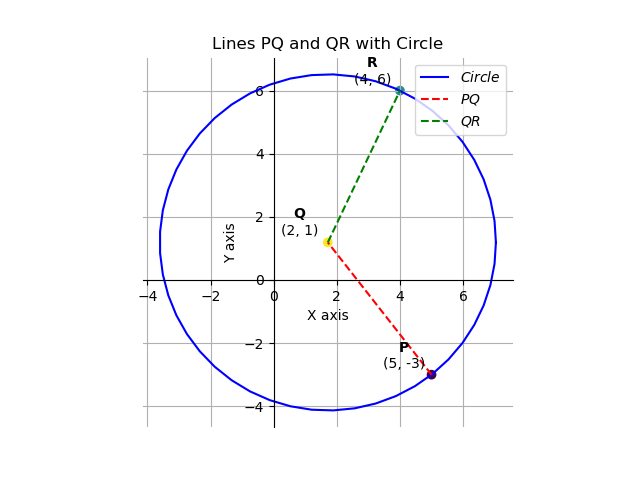
\includegraphics[width=10cm]{figs/Figure_1.png}
    \label{Point Q is Equidistant from P and R}
\end{figure}

\end{document}
